\begin{frame}{Simple Function Plot}
\begin{center}
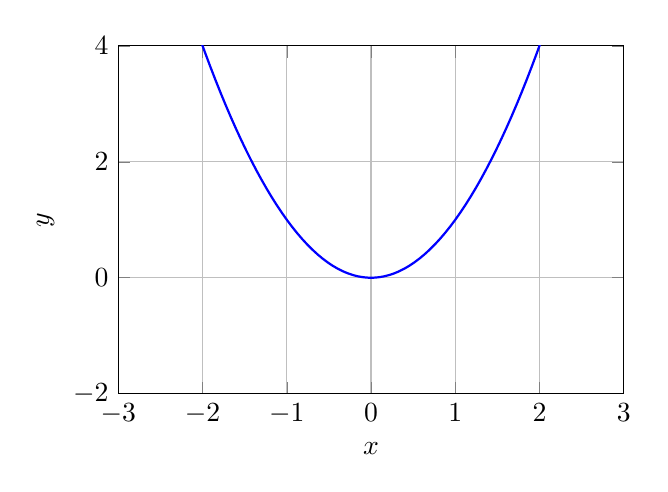
\begin{tikzpicture}
\begin{axis}[
    xlabel={$x$},
    ylabel={$y$},
    grid=both,
    xmin=-3, xmax=3,
    ymin=-2, ymax=4,
    width=8cm,
    height=6cm
]
\addplot[thick, blue, domain=-3:3, samples=100] {x^2};
\end{axis}
\end{tikzpicture}
\end{center}

\footnotesize
\texttt{\textbackslash addplot[thick, blue, domain=-3:3, samples=100] \{x\textasciicircum 2\};}
\end{frame}